\chapter{Evaluation}
\label{cha:evaluation}

\projectName{} is a prototypical implementation of a GDPR compliant solution of self-sovereign identity management
utilizing the blockchain. Since this project is a proof-of-concept rather than a working platform, we will do a critical
 review of the implementation and concept sections and outline the building blocks for future work.

\section{Core-Logic}
\label{sec:coreLogicEval}
Since the whole system is a prototype there are several improvements and alternative design choices that could increase
security and stability in the proposed system.

\subsection{Decentralized untrusted system}
\label{sec:untrustedSystem}
If we drop the principle of a private blockchain and let every provider write to the blockchain as well, we deescalate
the government as single point of failure.
To ensure further availability we could drop the discovery service and organize the discovery of an specific provider
in a distributed hash table. Since we want still off-blockchain communication we could think about a peer-to-peer
implementation which will completely decentralize the system. The final problem that still remains is how to establish
trust in a new user without having the government as a trusted party? Since we already considered the eID of the German
government as a verification mechanism we can take this to the next level by allowing the peers to retrieve identity
information from the eID directly. By doing so we would finally eliminate the government as needed, trusted party and
can relay only heavily on the trust already established in the certificate which signed eID of the user
\footnote{Of cause this certificate is still generated by the government but the government as such would be eliminated
as central component where requests would be routed though.}.

\begin{figure}
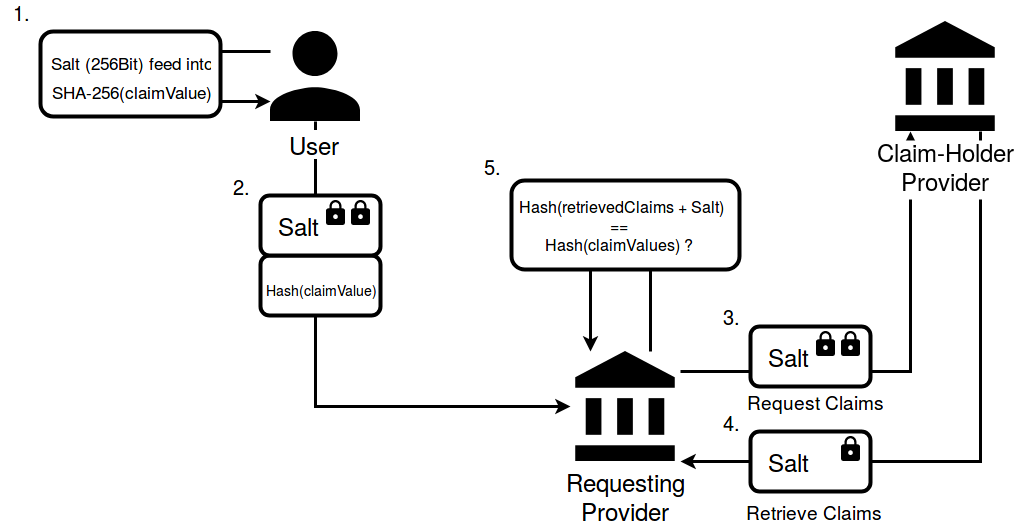
\includegraphics[width=0.7\textwidth]{concept/integrity.png}
\centering
\caption{Proposal of integrity check using layered encryption of the salt value.}
\label{fig:integrity}
\end{figure}

In such an untrusted system we need somehow verify the integrity of claims that are shared between providers.
Here we can use the fact that the user is holding his own signed claims in his local database.
On approving a permission contract he can send off-blockchain a hash of his claims to the provider requesting the claims,
to ensure that the claim holder does not tamper the claims when providing them to the requesting provider.
However, since the provider itself is untrusted he may try to brute-force the hash of the claims of the user and will
likely succeed if the hash is, for example, build over a boolean claim value. So we need to introduce a very strong salt.
Using SHA-256 to produce a 256 bit long hash value, a salt needs to be securely generated that is at least bigger
then 256 bits to ensure with 100\% certainty that a hash collision would exist
\footnote{For more information about hash collisions refer to the so called “birthday attack”
(\url{https://en.wikipedia.org/wiki/Birthday_attack}).}.
The implications are that even if a hash collision would be found by a malicious provider he has only a
50\% probability to hit the right boolean value. So basically he knows nothing. In figure \ref{fig:integrity}
step 1 is showing this creation of a salt. To now ensure that the provider can only check the integrity of
the user claims on retrieving the actual user claims, the user would encrypt the generated salt asymmetric with
the public key of the requesting provider and then again encrypt the salt again asymmetrically with the public key of
the provider that holds the claims (salt in step 2., layered encryption). The requesting provider needs the help of the
claim holder provider to decrypt the double encrypted salt and can then proceed by decrypting the salt with his own
private key (step 3 and step 4). By doing so we would additionally ensure that the claim holder provider can not craft
a hash collision salt and return the provider his salt with a faked claim value.  The requesting provider can now use
the plain salt to verify the hash over the boolean claim (step 5).

An completely untrusted system comes also with other drawbacks. We need to somehow enforce fairness and balance. Fairness ensures that if a provider requests claims from another provider it is somehow guaranteed that he either retrieves the claims or an equivalent amount of money. Balance would mean that requesting claims comes along with cost that the requester needs to pay. Indeed Ethereum is providing us with smart-contracts that can ensure this principles. However, GDPR is restricting us from saving either hashes nor encrypted claims in the blockchain, since if the key or the hashed preimage gets leaked, no one can remove this claims from the blockchain.

We should also think about how the “right to be forgotten” will be enforced. Of course we can simply introduce to do this manual by writing an email to the claim holder, but this is not the desired solution. It is a tricky point, since once a claim is shared, it can’t be simply revoked. We didn’t managed to find a suitable solution for this problem.  

\subsection{Closures are dangerous}
Remember that closures are boolean expressions build over a claim value, a logical comparator and a static value that is used to compare it to the claim value. Closures shell not expose the claim value. But this is not always the case. Closures are only hiding the claim value if the closure result is \textit{unlinkable} to the used claim value. However, building closure expressions over binary claim values and using the equals (EQ) or not equals (NEQ) operator will expose the claim value. A simple example is building a closure over the sex of a user: “SEX EQ ‘male’”. A provider can now use the closure result to relate it to the claim value of the user. If it evaluates to “true” the sex of the user is “male”, else it is “female”. We might also use EQ to guess claims of the user. Whenever EQ is used and the closure evaluates to “true”, the claim value of the user is exposed. As an implication we should only allow operators that relate to a higher anonymity set then two. Sadly we do not know which claims are “secure” to be used in closures and which are not, since also numbers or string values may only consist of binary values. 

\subsection{Security evaluation}
\label{sec:securityEvaluation}
To recap the security goals we managed to implement authenticity by appending a signature on each request. Integrity partially implemented. Each for each signed request the integrity is assured but we didn’t implement the integrity check over the claim values when requesting the claim values from the government service. Non-repudiation and accountability is ensured by populating each transaction trough the blockchain as well as attaching signatures to responses (e.g. claims or closures). We are privacy preserving in a pseudonym fashion were each user is identifiable by his unique Ethereum address. The encrypting process of closure is also providing forward secrecy were the session is a one-time session key and so never used again. However, we do not provide a mechanism of key change/key recovery of the RSA key-pair. A missing security goal is confidentiality since the communication between provider is not secured. TLS/SSL would help here to easily secure the communication.

\subsection{Summary}
The proposed backend is a proof-of-concept that identity in the blockchain can work even with law enforcements like GDPR. Still there are some improvements that could take into account when implementing the next version of this project. However, the proposed backend still offers some advantages that would be lost on completely decentralizing the system. The discovery service, as untrusted message broker and public key directory, is a simple and efficient solution to an peer-to-peer adaption of a client-server architecture. Further, we can simply trust each entry that comes from the government, since it is a trusted entity itself. This would not be possible in a complete untrusted system, where each request needs to validated by the user. Such an decentralized system would also have a hard time not to store hashes over claims in the blockchain to validate claim values, since each other location or transmission would not be tamper proof. 

\section{Database}
\label{sec:databaseEval}
As outlined in the previous Sections we chose couchbase as our database technology.(Ref. \ref{sec:database}) While this enabled us to directly work with the documents we were creating without the need for transforming them between database and code representations, it also brought problems with it aswell.
As described in further detail in previous parts (Ref. \ref{ssec:databaseDeployment}) we ant to reexamine the problems we had with this choice and our conclusions upon finishing the demonstrator. We will however try to focus on couchbase light, as that was our intended database framework all along, whenever it is possible and fall back to couchbase when not.

\subsection{Critique}
\label{ssec:databaseEvalCrit}
\begin{itemize}
\item \label{db_crit_one} \textbf{Working with couchbase from a developer perspective:}
While the team behind couchbase light promisses full mobile convergence between their upcoming solution and their current enterprise grade database, it is still possible that their definition of full mobile convergence might differ from ours.
For example the entire database interface might be structured in a different way, forcing us to either rewrite large parts of our code or create a custom interface to interact with their new interface. Furthermore a new and different implementation might, under specific circumstances, handle in an unexpected way.
While the methods might be the same, even a small difference in how certain methods are now being handled might break our code. Consider the possibility of a wrong implementation that still always delivered the intended result, simply because of how it is structured. Restructuring that interface might break the previously mentioned method.
In conclusion, going with a more established solution and taking the time to write methods for transforming data representations between database and core-logic structures might have been a more prudent decision.
\item \label{db_crit_two} \textbf{Working with couchbase from an operations standpoint:}
We would like to evaluate our current system, since it is as of yet unknown how we would handle a deployment of couchbase light.
During our work on \projectName{} we quickly realized that compared to other solutions, couchbase was very memory intensive. This has gotten up to a point where our VM was going into memory panic mode and shutting down other docker containers to release more memory and feed couchbases demand.
Additionally this behaviour disallowed us from truly testing our intended deployment of creating a seperate bucket for each entity and forcing us to fall back to a one bucket for all situation. Additionally the memory constraints prevented us from creating more indices to quicken queries.
This means that depending on current memory utilization levels some queries simply timed out and returned an error code instead of a result. This in turn made development for the frontend side of the project a little more communication intensive, to ask whether the frontend code itself was faulty or the database was running into
memory problems again.
Considering all these things we learned that in order to fully utilize couchbase and benefit from its schemaless design, we simply have to plan with a much higher memory allocation.
\item \label{db_crit_three} \textbf{Implications of couchbase for the actual userbase:}
Since couchbase light has not even been fully released yet, apart from pre-release test version, it carries a huge risk for the actual userbase. This is an unproven newly developed database framework coming into a marketplace that has already long been established with technologies that are now tried and true.
These established databases had their kinks ironed out years ago and had their fair share of security breaches. This means that all major flaws should now already be fixed or atleast replaced with a workaround. Couchbase light however has not had that amount of exposure yet, apart from laboratory or small scale internal tests yet.
Building on top of it demands a lot of trust into the developmental team behind couchbase light. More often than not potential security flaws are found by groups of it-experts with ill intentions and this could spill disaster for a system that is holding a persons entire identity information.\cite{biggestCyberSecurityDisasters2017}
Compared to security breaches occuring at services like the Playstation Network, Yahoo, iCloud, \projectName{} holds the entirety of your identity. The aforementioned services only hold part of your identity, and while a breach could still have catastrophic implications, atleast only partial identites were broken into.
All in all it seems like this burden is simply too much to bear. Considering that the company managing this system is then also responsible for any damage that any participant might incur. Lastly we would also like to mention that current digital services rendered by the german state are not fully secure as well.\cite{cccNewIdBroken,cccNewIdProblems}
\end{itemize}

\subsection{Evaluation}
\label{ssec:databaseEvalEval}
To summarize all above mentioned arguments, if we were to start from scratch we would reconsider our database choice strongly. We feel like solutions like SQLite, while not technically fitting because of our data layout, would still be a better contender.
To add on to the above mentioned reasons we didn't even try to run our intended system which consists of a single bucket for each entity. We mainly wanted to handle it this way to ensure that our implementation followed our design choices as closely as possible.
But since we had an enormous amount of memory limitation we had to abandon that notion. This is also probably why, with the knowledge we have gained during \projectName{}s developmental process, we would decide to go with a different database technology.